\setcounter{section}{4}
\setcounter{subsection}{4}
\setcounter{subsubsection}{3}
\setcounter{equation}{20}

\section{Elektronenzustände}
\subsection{Elektronenzustände beim Atom (Wiederholung)}
Ein Atom ist ein kugelsymmetrisches Gebilde, da der Kern ein kugelsymmetrisches Coulombfeld generiert.

\paragraph{Einzelelektron}
Zur Beschreibung eines Elektrons in einem Atom werden Quantenzahlen verwendet:
\begin{itemize}
	\item $n=1,2,3 \ldots$ grob die Energie
	\item $l=0,1,2,\ldots, n-1$ den Bahndrehimpuls $\sqrt{l(l+1)} \hbar $ 
	\item $s=\frac{1}{2}$ den Spin $\sqrt{s(s+1)} \hbar $ 
	\item $j= l \pm s$ den Gesamtdrehimpuls $\sqrt{j(j+1)} \hbar $
	\item $m_{i} = i\ldots -i$ mit $i=l,s,j$ die Projektion auf eine Vorzugsrichtung $m_{i} \hbar $
\end{itemize}

\paragraph{Mehrere Elektronen}
Atome mit mehreren Elektronen werden folgendermaßen beschrieben: 
\begin{itemize}
	\item $L = 0,1,2$ den Gesamtdrehimpuls $\Vec{L} = \sum_{i}^{} \Vec{l}_{i} $ $S,P,D$ 
	\item $S = 0,\frac{1}{2},1$ den Gesamtspin $\Vec{S} = \sum_{i}^{} \Vec{s}_{i} $ 
	\item $J= L+S , \ldots, L-S$ den Gesamtdrehimpuls $\Vec{J} = \Vec{L} + \Vec{S}$ 
	\item $m_{i} = i, \ldots, -i$ die Projektion $m_{i} \hbar $ mit $i= L, S, J$
\end{itemize}
Bei leichten Atomen gilt die Spin-Bahn-Kopplung.

\paragraph{Hund'sche Regeln}
\begin{figure}[H]
    \centering
    \incfig{vl11_abbildung_1}
    \caption{Elektronische Besetzung des Sauerstoffatoms.}
    \label{fig:vl11_abbildung_1}
\end{figure}

Die Hund'schen Regeln lauten
\begin{enumerate}
	\item Volle Schalen und Unterschalen tragen zu allen Drehimpulsen nicht bei
	\item Der Spin $S$ nimmt sein Maximum an. $S = \frac{1}{2} + \frac{1}{2} = 1$ bedeutet einen {Triplett-Zustand}.
	\item Der Drehimpuls $L = \left| \sum_{l}^{} m_{l}  \right|$ nimmt sein Maximum an. $L=1$ bedeutet, das Atom hat einen Dipol $\Vec{P}$. 
	\item $J= L+S$ falls Unterschale mehr als halb voll $\implies$ $J=2$. 
			${J}= L-S$ falls Unterschale weniger als halb voll\\
			$\implies$ Der Grundzustand des Sauerstoffs ist $^3\text{P}_{2}$. Die Notation folgt dem Schema $^{\text{2S + 1}} L_{J}$.
\end{enumerate}

\subsection{Elektronenzustände beim Molekül}

\subsubsection{Einzelelektronenzustände zweiatomiger Moleküle (\ce{H2}, \ce{O2}, \ce{N2}, \ldots)}
\begin{figure}[H]
	\centering
	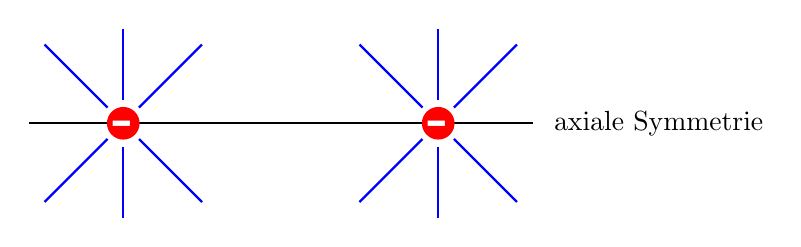
\begin{tikzpicture}
		\draw[thick] (-3.2,0)--(3.2,0);
		\draw[fill = red, color = red] (-2,0) circle (0.2);
		\draw[fill = red, color = red] (2,0) circle (0.2);
		\draw[thick, blue] (-2, 0.3) -- (-2, 1.2);
		\draw[thick, blue] (-2, -0.3) -- (-2, -1.2);
		\draw[thick, blue] (2, 0.3) -- (2, 1.2);
		\draw[thick, blue] (2, -0.3) -- (2, -1.2);

		\draw[thick, blue] (-2.2, 0.2) -- (-3, 1); 
		\draw[thick, blue] (-2.2, -0.2) -- (-3, -1); 
		\draw[thick, blue] (2.2, 0.2) -- (3, 1); 
		\draw[thick, blue] (2.2, -0.2) -- (3, -1); 

		\draw[thick, blue] (-1.8, 0.2) -- (-1,1);
		\draw[thick, blue] (-1.8, -0.2) -- (-1,-1);
		\draw[thick, blue] (1.8, 0.2) -- (1,1);
		\draw[thick, blue] (1.8, -0.2) -- (1,-1);
		\node[white] at (-2,0) {\huge\textbf{-}};
		\node[white] at (2,0) {\huge\textbf{-}};
		\node at (4.8,0) {axiale Symmetrie};
	\end{tikzpicture}
\end{figure}
\begin{itemize}
	\item Aus der Linearkombination von Atomorbitalen bildet man Molekülorbitale.
	\item Die verfügbaren Elektronen werden in die Molekülorbitale so eingebaut, dass diese ihrer energetischen Reihenfolge nach aufgefüllt werden unter Berücksichtigung des Pauli-Prinzips
	\item Hund'sche Regeln: Bei der Besetzung energetisch entarteter Orbitale wird zunächst jedes Molekülorbital einfach besetzt, bevor Zweifachbesetzung erfolgt. Dabei ist die Anordnung mit parallelen Spins bevorzugt.
\end{itemize}
Vernachlässigt wird Schwingung und Rotation.

\textbf{Quantenzahlen}
\begin{itemize}
	\item $n = 1,2,3$ wie früher
	\item Aufgrund der Abweichung von der Zentralsymmetrie ist die Drehimpulsquantenzahl $l$ keine gute Quantenzahl mehr, jedoch gibt es noch $m_{l}$ bezogen auf die Kernverbindungslinie $l_{z} = m_{l} \hbar $
		\begin{itemize}
			\item $m_{l} = l, l-1 ,\ldots, -l$ 
			\item $m_{l} $ positiv $\to $ Elektron läuft rechts herum
			\item $m_{l} $ negativ $\to $ Elektron läuft links herum
		\end{itemize}
		Die Wirkung des elektrischen Feldes auf ein präzedierendes Elektron ist unabhängig von dessen Umlaufsinn.
		\begin{itemize}[label= $\to$]
			\item Nur der Betrag von $m_{l}$ ist wichtig.
			\item Die neue Quantenzahl $ \lambda = \left| m_{l} \right| = 0, 1, 2, \ldots$ wird eingefürt. Sie ist zweifach entartet für $\left| m_{l} \right| \ge 1.$
		\end{itemize}
\end{itemize}

\begin{table}[htpb]
	\centering
	\caption{Symbole zur Quantenzahl $\lambda$.}
	\label{tab:label}
	\begin{tabular}{|l|c|c|c|c|}
	\hline
	$m_{l}$   & $0$       & $\pm 1$& $\pm 2$   & $\pm 3$     \\
	\hline
	\hline
	$\lambda$ & $0$       & $1$    & $2$       & $3$         \\
	\hline
	Symbol    & $ \sigma$ & $ \pi$ & $ \delta$ & $ \varphi$  \\
	\hline
	\end{tabular}
\end{table}
Es gilt $m_{s}= \pm \frac{1}{2}$ relativ zur Vorzugsachse. Damit können $ \sigma$-Zustände zwei Elektronen aufnehmen und alle anderen vier.\\

\paragraph{\thesubsubsection.a) Getrennte Atome $A$ und $B$}~\\
Man benutzt die Quantenzahlen, die in völlig getrennten Atomen gelten.


\textbf{Beispiel:} $ \sigma 1 \mathrm{s}_{A}$ mit dem 1s-Orbital von Atom $A$ und $\sigma 2 \mathrm{p}_{B}$ mit dem 2p-Orbital von Atom $B$.
\begin{important}
	Die Benennung der Zustände erfolgt nach dem Schema $\lambda nl$. 
\end{important}
Man kann die Orbitale auch umgekehrt kennzeichnen.

\textbf{Beispiel:} $3\mathrm{d} \pi$-Elektron. Das Elektron hatte ursprünglich $n=3$, $l=2$ und ist jetzt in einem $\lambda=1$ Orbital

\textbf{Symmetrie}: Als gerade (Index 'g') oder ungerade (Index 'u') bezeichnet man Orbital-Wellenfunktionen, je nachdem ob sie symmetrisch oder antisymmetrisch relativ zu einem Symmetriezentrum des Moleküls sind. Bspw. ist $ \sigma_{\mathrm{g}}$ eine gerade Funktion mit $ \lambda =0$.

\textbf{Beispiel:} Bilde aus zwei 1s-Orbitalen von zwei getrennten Atomen $A$ und $B$ durch Linearkombination ein Molekülorbital:
$$
\begin{aligned}
	\sigma_{\mathrm{g}} 1\mathrm{s} &= \frac{1}{\sqrt{2} } \left( 1\mathrm{s}_{A} + 1\mathrm{s}_{B}\right) \quad \text{bindend} \\
	\sigma_{\mathrm{u}} 1\mathrm{s} &= \frac{1}{\sqrt{2} } \left( 1\mathrm{s}_{A} - 1\mathrm{s}_{B} \right) \quad \text{antibindend} \to \sigma^{*} \\
\end{aligned}
$$ 
Die Markierung $*$ steht für antibindende Zustände.

\subsubsection{Mehrelektronenzustände und elektrische Gesamtzustände}
Die Molekülachse entspricht der starken Vorzugsrichtung der elektronischen Achse.
\begin{itemize}
	\item Gegenseitige Kopplung der Elektronen muss beachtet werden um zu einer Charakterisierung des Gesamtzustandes zu kommen
	\item Drehimpulse der inneren Elektronen in abgeschlossenen Schalen kompensieren sich
\end{itemize}

\paragraph{1. Bahndrehimpulse}~\\
\begin{minipage}{0.5\linewidth}
	\centering
	\includegraphics[width=\textwidth]{./figures/VL11_Abbildung_2.tikz}
	\captionof{figure}{Bahndrehimpulse der Elektronen.}
	\label{fig:vl11_bahndrehimpulse}
\end{minipage}
\begin{minipage}{0.5\linewidth}
	Kopplung der $l_{i}$ untereinander zu $L$ ist meistens schwächer als der einzelnen Elektronen an das axiale Feld der Kerne. 
	$$
	\begin{aligned}
		\Lambda &= \left| \Sigma_{i} \lambda_{i}  \right| = 0,1,2,\ldots \quad \Sigma, \Pi, \Delta \\
		L_{z} &= \pm \Lambda \hbar  
	\end{aligned}
	$$ 
\end{minipage}

\paragraph{2. Spins}~\\

\begin{minipage}{0.5\linewidth}
	\centering
	\includegraphics[width=\textwidth]{./figures/VL11_Abbildung_3.tikz}
	\captionof{figure}{Gesamtspin mit Quantenzahl $\Sigma$.}
	\label{fig:vl11_gesamtspin}
\end{minipage}
\hspace{0.05\linewidth}
\begin{minipage}{0.45\linewidth}
	Die Spins koppeln zum Gesamtspin
	$$
	S_{z} = \Sigma \hbar \quad \text{mit} \quad \Sigma = S, S-1, \ldots, -S.
	$$ 
	Er hat Multiplizität $2S + 1 $.\\
	Durch die Orientierung der Bahndrehimpulse längs der Molekülachse wird die Molekülachse auch zu einer \textbf{magnetischen Achse}.

	Der Gesamtspin präzediert. Die Projektion des Spins hat also eine physikalische Bedeutung.

\end{minipage}

\paragraph{3. Gesamtdrehimpuls der Elektronen}~\\
\begin{minipage}{0.4\linewidth}
	\centering
	\includegraphics[width=\textwidth]{./figures/VL11_Abbildung_4.tikz}
	\captionof{figure}{Gesamtdrehimpuls der Elektronen}
	\label{fig:vl11_gesamtdrehimpuls_elektronen}
\end{minipage}
\hfill
\begin{minipage}{0.5\linewidth}
	$ \Omega$ entspricht dem Gesamtdrehimpuls der Elektronenhülle (nicht des Gesamtmoleküls). $ \Sigma$ und $ \Lambda$ können gleich oder entgegengesetzt gerichtet sein
	$$
	\Omega = \left| \Lambda + \Sigma \right|, \quad \Sigma= S, S-1, \ldots , -S
	$$
	Infolge der Spin-Bahn-Kopplung zwischen $\Vec{L}$ und $\Vec{S}$ spaltet also jeder zu einem bestimmten Wert von $ \Lambda$ gehörende Term in ein Multiplett von $ 2S + 1$ Termen auf.
	\begin{important}
		\textbf{Nomenklatur:} $ ^{2S+1}\Lambda_{ \Omega}$\\
	\end{important}

\end{minipage}

\paragraph{Beispiel} 
	Ein Zustand ist durch die Konfigurationssymbole bezeichnet. 
	Mit drei 3 Valenzelektronen ist ein Zustand bspw. $$(2\mathrm{p} \pi) (3\mathrm{s}\sigma)(3\mathrm{d}\pi)~^{4}\Delta_{3 /2}.$$

\begin{itemize}
	\item für den Bahndrehimpuls gilt $ \Lambda =2$ da $ \Delta$.
	\item für den resultierenden Spin $2S +1 = 4$ $\to $ $S = \frac{3}{2}$ .
	\item $\Omega = \left| \Lambda + \Sigma \right| = \frac{3}{2}$, es folgt der Zustand $^{4}\Delta_{3 /2}$ mit $\Sigma= -\frac{1}{2}$. Andere mögliche Zustände je nach Spinstellung ($\Sigma = \frac{3}{2}, \frac{1}{2}, -\frac{1}{2}, -\frac{3}{2}$) sind
		$$
		^{4}\Delta_{7 /2},~^{4}\Delta_{5 /2},~^{4}\Delta_{3 /2},~^{4}\Delta_{1/2}
		$$
		\begin{itemize}
			\item Die meisten Moleküle haben $^{1}\Sigma_{0}$ $\to $ diamagnetisch
			\item Beachte: Der Gesamtdrehimpuls $J$ setzt sich aus den Elektronendrehimpulsen $\Omega$ und dem Hanteldrehimpuls $N$ zusammen: $\Vec{J} = \Vec{N} + \Vec{\Omega}$. Bei allgemeinen konkurierenden Magnetfeldern gibt es verschiedene Kopplungsfälle, nach Hund gibt es die A,B,C,D,E-Fälle. Hier wurde Fall A besprochen.
		\end{itemize}
\end{itemize}

\paragraph{4. Symmetriebetrachtung}~\\

\begin{minipage}{0.4\linewidth}
	\centering
	\includegraphics[width=\textwidth]{./figures/VL11_Abbildung_5.tikz}
	\captionof{figure}{Symmetriebetrachtung}
	\label{fig:vl11_symmetriebetrachtung}
\end{minipage}
\hfill
\begin{minipage}{0.5\linewidth}
	\begin{enumerate}
		\item $ \Sigma^{+}$ und $\Sigma^{-}$ \\
			'$+$' bedeutet, dass die Elektronen-Wellenfunktion ihr Vorzeichen bei Spiegelung an der Ebene $E$ beibehält
		\item $\Sigma_{\text{g}}$ und $\Sigma_{\text{u}}$ g,u $\to $ Parität\\
			'g' bedeutet Elektronen-Wellenfunktion behält ihr Vorzeichen bei Spiegelung am Zentrum $Z$
	\end{enumerate}
\end{minipage}


